\documentclass{article}
\usepackage{tikz}
\usetikzlibrary{positioning}

\begin{document}
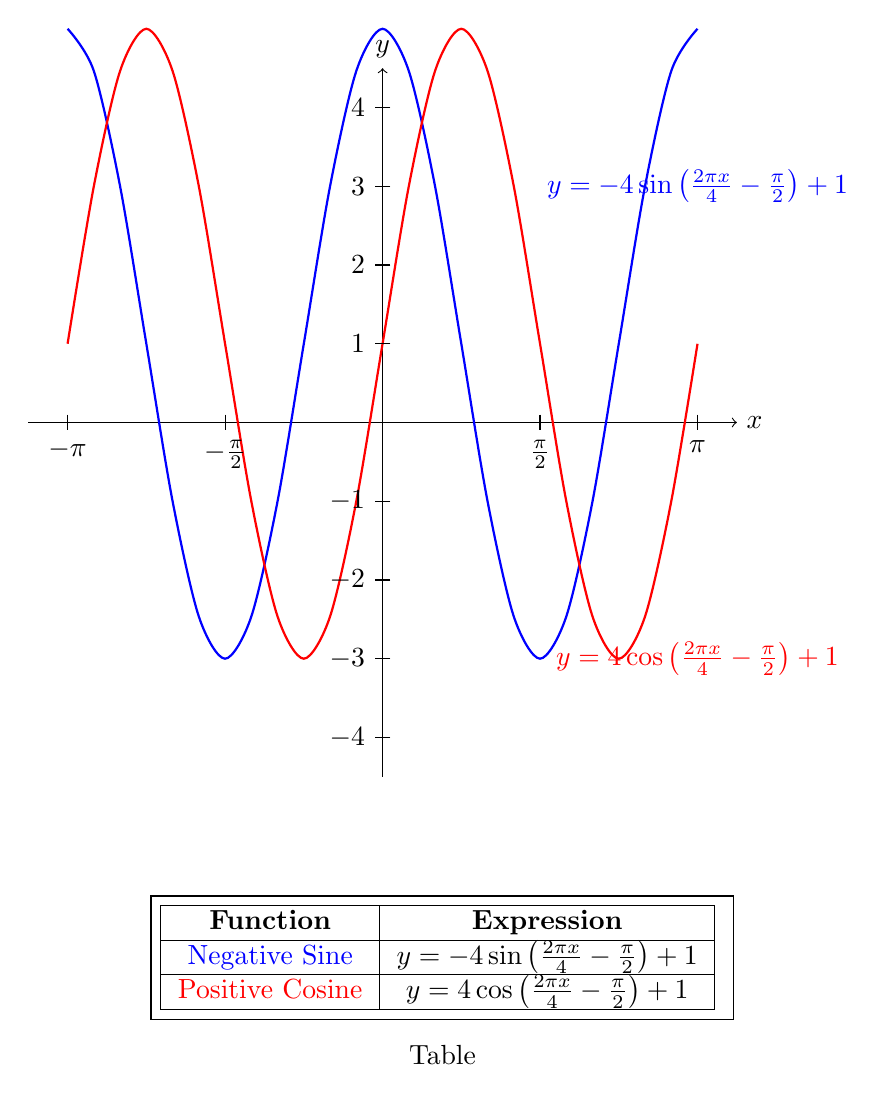
\begin{tikzpicture}
  \draw[->] (-4.5,0) -- (4.5,0) node[right] {$x$};
  \draw[->] (0,-4.5) -- (0,4.5) node[above] {$y$};

  % Function y = -4 * sin(2π * x / 4 - π/2) + 1
  \draw[domain=-4:4, smooth, variable=\x, blue, thick] plot ({\x}, {-4*sin(360*\x/4 - 90) + 1});
  \node[blue] at (4, 3) {$y = -4 \sin\left(\frac{2\pi x}{4} - \frac{\pi}{2}\right) + 1$};

  % Function y = 4 * cos(2π * x / 4 - π/2) + 1
  \draw[domain=-4:4, smooth, variable=\x, red, thick] plot ({\x}, {4*cos(360*\x/4 - 90) + 1});
  \node[red] at (4, -3) {$y = 4 \cos\left(\frac{2\pi x}{4} - \frac{\pi}{2}\right) + 1$};

  \foreach \x/\xtext in {-4/{-\pi}, -2/{-\frac{\pi}{2}}, 2/{\frac{\pi}{2}}, 4/{\pi}}
    \draw (\x,0.1) -- (\x,-0.1) node[below] {$\xtext$};
  \foreach \y/\ytext in {-4/{-4}, -3/{-3}, -2/{-2}, -1/{-1}, 1/{1}, 2/{2}, 3/{3}, 4/{4}}
    \draw (0.1,\y) -- (-0.1,\y) node[left] {$\ytext$};

  % Table
  \node[draw, fill=white, align=center, below=1.5cm of current bounding box.south] (table) {
    \begin{tabular}{|c|c|}
      \hline
      \textbf{Function} & \textbf{Expression} \\
      \hline
      \textcolor{blue}{Negative Sine} & $y = -4 \sin\left(\frac{2\pi x}{4} - \frac{\pi}{2}\right) + 1$ \\
      \hline
      \textcolor{red}{Positive Cosine} & $y = 4 \cos\left(\frac{2\pi x}{4} - \frac{\pi}{2}\right) + 1$ \\
      \hline
    \end{tabular}
  };
  \node[below=0.2cm of table] {Table};

\end{tikzpicture}
\end{document}